\section{Motivation}
\label{sec:motivation}

In this section, we examine the gap between high application demands and limited
wide-area bandwidth. We then show that neither manual policies nor
application-specific optimizations solve the problem.

\subsection{Wide-area Streaming Applications}
\label{sec:wide-area-streaming}

\paraf{Video Surveillance.} We envisage a city-wide monitoring system that
aggregates camera feeds---from stationary ground cameras and moving aerial
vehicles---and analyzes video streams in real-time for surveillance, anomaly
detection or business intelligence~\cite{oh2011large}. Traditionally, video
analysis requires human involvement. Recent advances in computer vision and deep
learning have dramatically increased the accuracy for automatic visual scene
analysis, such as pedestrian detection~\cite{dollar2012pedestrian}, vehicle
tracking~\cite{coifman1998real}, and facial recognition to locate people of
interest~\cite{Lu:2015:SHF:2888116.2888245, parkhi2015deep}. While some
surveillance cameras use dedicated links, an increasing number of surveillance
systems, such as Dropcam~\cite{dropcam} and Vigil~\cite{zhang2015design}, use
the public Internet and wireless links to reduce the cost of deployment and
management.

% \para{High-frequency IoT Sensors:} Although environmental sensors used to be
% slow and not data-intensive~\cite{atzori2010internet}, increasingly,
% high-frequency, high-precision sensors are deployed. For example, uPMUs
% monitor the electrical grid with a network of 1000 devices; each produces 12
% streams of 120 Hz high-precision values accurate to 100 ns. This amounts to
% 1.4 million points per second~\cite{andersen2016btrdb}.

\para{Infrastructure Monitoring.} Large organizations today are managing
10--100s of data centers (DCs) and edge clusters
worldwide~\cite{calder2013mapping}. This geo-distributed infrastructure
continuously produces large volumes of data such as data access logs, server
monitoring logs, and performance counters~\cite{alspaugh2014analyzing,
  pu2015low, vulimiri2015global}. While most log analysis today runs in a batch
mode on a daily basis, there is a trend towards analyzing logs in real time for
rapid optimization~\cite{rabkin2014aggregation}. For example, CDNs can improve
the overall efficiency by optimizing data placement if the access logs can be
processed in real time. \fixme{one or two sentences about industrial IoT (factory
monitoring), e.g., GE. Citing some news articles is enough.}

%% ~\cite{xu2009detecting} We generated the HDFS logs by setting up a Hadoop
%% cluster on 203 EC2 nodes and running sample Hadoop map-reduce jobs for 48
%% hours, generating and processing over 200 TB of random data. We collected
%% over 24 million lines of logs from HDFS.

% We consider the practical issues with deploying these applications in the
% wide-area. Our stand is that these applications face a bigger network
% challenge.  Data generated from the edge often fail to be delivered to the
% processing site because of the scarce and variable bandwidth capacity in the
% wide-area. Once they arrive, existing stream processing systems can easily
% manage a large cluster and perform data analytics at real-time.

\subsection{Wide-area Bandwidth Characteristics}
\label{sec:wide-area-bandwidth}

WAN bandwidth is insufficient and costly, as demonstrated by recent WAN-aware
systems~\cite{hsieh17gaia, pu2015low, vulimiri2015wananlytics,
  vulimiri2015global}. Using Amazon EC2 as a case study, the WAN bandwidth
capacity is 15x smaller than their LAN bandwidth on average, and up to 60x
smaller in the worst case~\cite{hsieh17gaia}. In terms of pricing, the average
WAN bandwidth cost is up to 38x of the cost of renting two
machines~\cite{amazon2017pricing, hsieh17gaia}.

In addition to the scarcity and cost, the large variability of WAN bandwidth
also affects streaming workloads. We conducted a day-long measurement with
iPerf~\cite{iperf3} to study the pair-wise bandwidth between four Amazon EC2
sites. \fixme{specify the four sites.} The results show large variance in all pairs---
\autoref{fig:bw} is one
such pair. \fixme{do the results hold for all pairs? We did not pick the worst
pair. Say we have results for all pairs in appendix.} There are occasions when
the available bandwidth is below 25\% of the
maximum bandwidth.

\begin{figure}
  \centering
  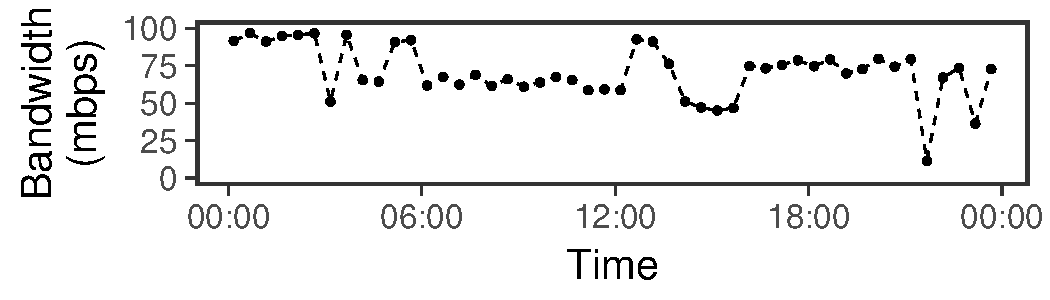
\includegraphics[width=0.9\linewidth]{figures/aws-variation.pdf}
  \caption{Bandwidth variations throughout the day between Amazon EC2 sites
    (from Ireland to California).}
  \label{fig:bw}
\end{figure}

The back-haul links between EC2 sites are better---if not at least
representative---in comparison to general WAN links. Similar scarcity and
variations have been reported in wireless networks~\cite{biswas2015large},
broadband access networks~\cite{grover2013peeking, sundaresan2014bismark} and
cellular networks~\cite{nikravesh2014mobile}. \fixme{what about clients (your laptops)
to DC. Say for normal users (e.g., you deploy a Dropcam at home and run analytics
at EC2). The situation could be worse.}

\subsection{The Case for a System Approach}
\label{sec:making-case-sys-approach}

To address bandwidth limitation, existing solutions use manual policies and
application-specific solutions. We discuss their drawbacks to motivate a system
approach. \fixme{implying others, e.g., JetStream, are not a system approach. Need
a different subtitle, e.g., Motivation for AWStream}

\para{Manual polices are sub-optimal.} While existing systems such as
JetStream~\cite{rabkin2014aggregation} and DASH~\cite{sodagar2011mpeg} \fixme{is DASH
manual?} allow
adaptation, they require developers to write manual policies. We illustrate the
problems with manual policies using an example~\cite{rabkin2014aggregation} \fixme{Be
careful here. Need to be specific, e.g., which section/page of JetStream}:
\textit{if bandwidth is insufficient, switch to sending images at 75\% fidelity,
  then 50\% if there still isn't enough bandwidth. Beyond that point, reduce the
  frame rate, but keep the image fidelity.}

First, this policy is not accurate.  Developers write such rules based on
heuristics and don't back them up with measurements. Images with 75\% fidelity
do not necessarily lead to 75\% application accuracy. In terms of bandwidth,
naively one would think that reducing the frame rate by half will also half the
data rate. But if video encoding such as H.264~\cite{richardson2011h} is used, a
reduction in frame rate increases the inter-frame difference and creates
P-frames with larger sizes. \hyperref[fig:app-specific]{Fig.~3e} shows that when
reducing the frame rate to 33\% (from \(30~\text{FPS}\) to \(10~\text{FPS}\)),
the bandwidth demand can still be more than 50\%.

Second, it is not scalable to specify rules one by one. When the policy involves
multiple dimensions or developers desire a fine-grain control, the policy will
end up with too many rules.  Writing such rules manually is a tedious and
error-prone process. \fixme{Mention profiling is also a pain. Need better tools for
the entire process.}

Lastly, this abstraction is too low-level. It forces developers to study and
measure the impact of individual operations, prohibiting its wide adoption in
practice.

\para{Application-specific optimizations do not generalize.} Because each
application has a different performance metric, relies on different features,
and targets different data distributions, a fine-tuned policy for one
application will often work poorly for others. \fixme{DASH should be moved to this
section.}

Analytical applications have their own goals, entailing different optimization
metrics and different algorithms. In video analytics, for instance, object
detection algorithms depend on the edge
information~\cite{canny1986computational, lowe2004distinctive, viola2001rapid}
while object tracking~\cite{allen2004object} works best when the inter-frame
difference is small. The former is sensitive to resolution changes while the
latter frame to rate changes.

\begin{figure*}
  \centering
  \includegraphics[width=0.9\linewidth]{figures/motiv-app-specific.pdf}
  \caption{The measured bandwidth and application accuracy for two video
    analytics applications.  (1) Different degradation strategies have different
    impacts on accuracy, e.g., degrading frame rate in (a) vs.\,degrading
    resolution in (b).  (2) The same degradation strategy has different impacts
    on different applications, e.g., degrading frame rates works well for
    stationary camera (a), but not well for mobile camera (e). (c-g) shows
    example measurement frames. \fixme{this example is not described in text.}}
  \label{fig:app-specific}
\end{figure*}

Similar applications face different data distributions, as shown in
\autoref{fig:app-specific} between stationary cameras detecting pedestrians and
mobile cameras recognizing objects. For stationary cameras, when we consider the
slow walking speed of pedestrians, a high frame rate is not necessary. But
high-resolution images are crucial because these surveillance cameras are far
away from the targets. In the mobile camera case, because the cameras move,
reducing the frame rate introduces significant errors.

%%% Local Variables:
%%% mode: latex
%%% TeX-master: "awstream"
%%% End:
